\documentclass[10pt,twocolumn,letterpaper]{article}

\usepackage{cvpr}
\usepackage{times}
\usepackage{epsfig}
\usepackage{graphicx}
\usepackage{amsmath}
\usepackage{amssymb}
\usepackage{booktabs}
\usepackage{algorithm}
\usepackage{algorithmic}
\usepackage{tabularx}
\usepackage{multirow}

\usepackage[pagebackref=true,breaklinks=true,letterpaper=true,colorlinks,bookmarks=false]{hyperref}

\cvprfinalcopy

\def\cvprPaperID{****}
\def\httilde{\mbox{\tt\raisebox{-.5ex}{\symbol{126}}}}

\ifcvprfinal\pagestyle{empty}\fi

\begin{document}

%%%%%%%%% TITLE
\title{Financial Computing Power Network: A Study on Next-Generation IT Infrastructure Layout Optimization for ICBC}

\author{Xiaoquan Zhi\\
Student\\
Tianjin Universtiy\\
Tianjin
\and
Jianing Zhao\\
Student\\
Tianjin Universtiy\\
Tianjin
\and
Yihan Wang\\
Student\\
Tianjin Universtiy\\
Tianjin
\and
Pengyu Wang\\
Student\\
Tianjin Universtiy\\
Tianjin
}

\maketitle

%%%%%%%%% ABSTRACT
\begin{abstract}
As the digital economy deepens, data has become a core factor of production in the banking industry, driving profound transformations in business and management models. As an industry leader, the Industrial and Commercial Bank of China (ICBC) is actively advancing into the "Digital 2.0" phase, driven by the dual wheels of technology and data. Against this backdrop, traditional IT infrastructure models are struggling to meet the stringent demands of financial services in terms of cost, latency, efficiency, and compliance. This paper first reviews the evolution of banking IT infrastructure from mainframes to cloud computing, identifying the bottlenecks of the current centralized cloud architecture in addressing new, ubiquitous, real-time, and intelligent financial demands. Building on this, we propose a forward-looking novel information infrastructure: the Financial Computing Power Network (F-CPN). This network aims to integrate and intelligently orchestrate distributed computing resources across the cloud, edge, and end-devices. The core of this work focuses on the key scientific problems in F-CPN layout optimization---resource allocation and cost control---abstracting them into two major classes of combinatorial optimization models: (1) a model for maximizing demand coverage under budget constraints, and (2) a model for minimizing total deployment costs while satisfying all demand. Given the computational complexity of such NP-Hard problems, this paper further explores the potential of quantum computing as a disruptive solution paradigm. The goal is to provide a solid theoretical basis and a feasible practical methodology for the scientific planning and forward-thinking technological layout of ICBC's next-generation IT infrastructure.
\end{abstract}

\textbf{Keywords} FinTech; Computing Power Network; Combinatorial Optimization; Quantum Computing; Digital Transformation in Banking

%%%%%%%%% BODY TEXT
\section{Introduction}

\subsection{A Review of Banking IT Infrastructure Evolution and Its Bottlenecks}

The symbiotic relationship between financial services and information technology has been a defining feature of the modern economy. Throughout its history, banking IT infrastructure has served as the central nervous system of the industry, dictating the pace of innovation, shaping customer interactions, and defining the very boundaries of business operations. The imperative for continuous digital transformation, as extensively documented in recent literature \cite{firat2023future}, compels a critical examination of this infrastructure's evolutionary trajectory. This evolution is not merely a story of technological replacement but a reflection of a profound principle often summarized by Conway's Law: an organization's IT architecture inevitably mirrors its business and communication structure. The journey from highly centralized, product-centric models to today's customer-centric, ecosystem-driven landscape is directly mapped onto the four major stages of its underlying technology stack.

\begin{figure*}[htbp]
\begin{center}
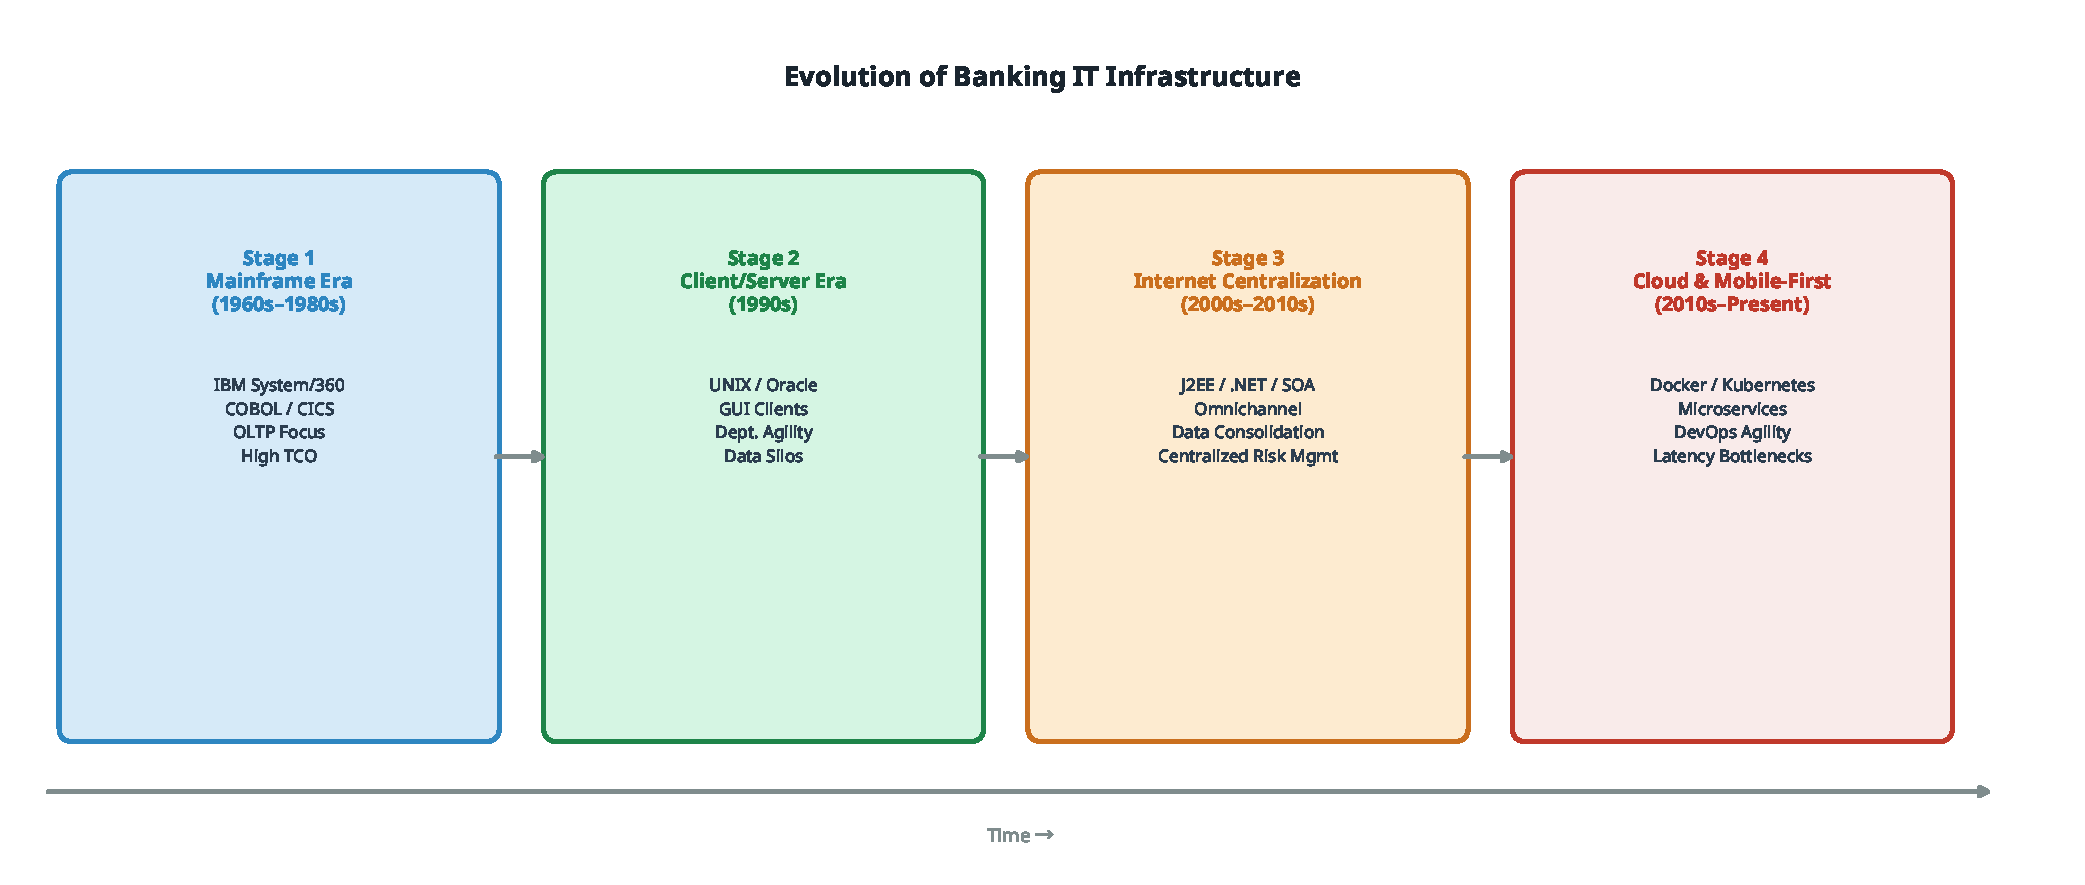
\includegraphics[width=0.9\linewidth]{fig1_evolution_timeline.pdf}
\end{center}
   \caption{Evolution of Banking IT Infrastructure}
\label{fig:evolution}
\end{figure*}

\begin{itemize}
    \item \textbf{Stage 1: The Mainframe Era---The Fortress of Transactional Integrity (1960s-1980s).} The dawn of banking automation was dominated by the mainframe, epitomized by platforms like the IBM System/360. This architecture was a direct reflection of the bank's hierarchical structure. Its core purpose was to be the ultimate \textbf{System of Record}, providing unparalleled reliability, consistency, and security for high-volume Online Transaction Processing (OLTP). Technologies like COBOL for business logic and CICS for transaction management created a robust but monolithic fortress. However, this strength was also its critical weakness. These proprietary, vertically integrated systems resulted in an extremely high Total Cost of Ownership (TCO) and created what can be termed "architectural rigidity" \cite{ross2019designed}. Business processes were hard-coded, data was locked within VSAM files, and any change required long, risky, and expensive development cycles. The mainframe's "information silo" nature was not just a technical artifact but a barrier to business agility, making it ill-suited to respond to the burgeoning demand for diversified financial products.
    
    \item \textbf{Stage 2: The Distributed Client/Server Era---A Push for Agility and its Perils (1990s).} The proliferation of personal computers and local area networks (LANs), driven by Moore's Law, triggered a paradigm shift. Banks embraced the Client/Server architecture to escape the mainframe's rigidity and cost. Processing was decentralized: presentation logic moved to client-side graphical user interfaces (GUIs), while business logic was handled by more affordable departmental servers running on open systems like UNIX with relational databases (e.g., Oracle, Sybase). This shift successfully empowered business units and improved the user experience. However, this newfound flexibility came at a steep price. The rapid, uncoordinated adoption led to a fragmented landscape of "islands of automation." The lack of robust middleware and standardized data models resulted in severe data integrity and consistency challenges, effectively creating new, more numerous "data silos" \cite{ometov2022survey}. Integrating these heterogeneous systems was a complex and brittle process, undermining the goal of a unified view of the customer.
    
    \item \textbf{Stage 3: The Internet Data Centralization Era---Rebuilding the Core for Omnichannel (2000s-2010s).} The explosive growth of internet and mobile banking created an urgent business driver: the need for a seamless, consistent \textbf{omnichannel experience}. A customer expected the same data and services whether they were at a branch, on a website, or using a mobile app. This forced a strategic reversal of the fragmentation of the previous era. The industry undertook massive "data centralization" projects, often building upon N-tier architectures and nascent Service-Oriented Architectures (SOA) using platforms like J2EE and .NET. The goal was to re-establish a "single source of truth" by consolidating disparate databases and application logic back into enterprise-level data centers. This recentralization was successful in providing a unified customer view and enabling centralized risk management, marking a significant milestone in the digital journey of banking \cite{firat2023future}. Yet, in doing so, it created a new form of centralized dependency, setting the stage for the next wave of disruption.
    
    \item \textbf{Stage 4: The Cloud \& Mobile-First Era---The Apex of Centralization and Its Emerging Fractures (2010s-Present).} Cloud computing, with its promise of on-demand elasticity, utility-based pricing (OpEx vs. CapEx), and unprecedented agility through DevOps, became the de facto standard for new application development. Banks built powerful private clouds and cautiously adopted hybrid models, leveraging virtualization, containers (Docker, Kubernetes), and microservices to accelerate time-to-market. While this model excels at large-scale data processing and flexible resource allocation, its purely centralized nature has revealed critical fractures when confronted with the demands of a truly ubiquitous, real-time, and intelligent "Digital 2.0" world. These are not minor issues but fundamental bottlenecks:
\end{itemize}

\begin{enumerate}
    \item \textbf{The Physical Latency Bottleneck:} The speed of light is a non-negotiable physical constraint. For latency-sensitive financial applications, this is a critical barrier. Round-trip times (RTT) to a distant central cloud can easily range from 50 to 150 milliseconds. This is unacceptable for services like real-time fraud detection during a transaction, interactive VTM video sessions, or high-frequency trading, which demand sub-10 millisecond response times.
    \item \textbf{The Data Gravity and Bandwidth Bottleneck:} The digital bank is a data factory, generating massive, often petabyte-scale, streams of unstructured data from sources like HD video surveillance, IoT sensors in branches, and chatbot logs. Transporting this deluge of raw data to a central cloud for processing is not only economically prohibitive due to network bandwidth and cloud egress costs but also highly inefficient. The principle of "data gravity"---the idea that data is hard to move---dictates that computation should move to the data, not the other way around.
    \item \textbf{The Data Sovereignty and Compliance Bottleneck:} A new generation of stringent data protection regulations, such as Europe's GDPR and China's own Data Security Law (DSL) and Personal Information Protection Law (PIPL), mandate data sovereignty. These laws impose strict rules on the cross-border transfer and localization of sensitive personal and financial data. A centralized cloud architecture, especially one involving public cloud regions, presents significant compliance risks and complexities, often making it legally impossible to process certain data outside of its geographical origin.
    \item \textbf{The Intelligent Application Bottleneck:} The future of banking services is intelligent, powered by Artificial Intelligence (AI). While AI model \textit{training} can leverage the massive power of the central cloud, AI \textit{inference}---the real-time application of these models---is most effective at the edge. Deploying inference workloads closer to the user enables immediate, context-aware services like real-time facial recognition for VIP access, natural language processing for voice commands at an ATM, or proactive customer assistance based on in-branch behavior analysis. Relying on the cloud for such inference introduces unacceptable latency and renders these smart applications impractical.
\end{enumerate}

\subsection{Research Objectives: Building and Optimizing the F-CPN}

The identified bottlenecks of the centralized cloud model are not mere incremental challenges but systemic limitations, indicating that the architecture is approaching an inflection point. To transcend these barriers, a paradigm shift is required. Drawing inspiration from the emerging concept of the Computing Power Network (CPN), which envisions a nationwide infrastructure for on-demand, orchestrated computing resources \cite{liu2023computing}, this paper proposes a domain-specific adaptation for the financial sector: the \textbf{Financial Computing Power Network (F-CPN)}.

The vision of F-CPN is to architect a fluid, three-tiered computational fabric that intelligently orchestrates resources across the entire institutional footprint---from central cloud data centers to edge servers located in branches, and even to the end-user devices. This is not merely a technical reconfiguration; it is a strategic imperative to design a business architecture for sustained digital success \cite{ross2019designed}. The value of this vision is best illustrated through concrete banking scenarios:

\begin{itemize}
    \item \textbf{Case Study 1: The "Smart Branch" Transformation.} Consider a next-generation bank branch equipped with VTMs (Virtual Teller Machines), biometric authentication, and AI-powered customer analytics. In a traditional cloud model, the high-definition video stream from a VTM session would travel hundreds of kilometers to a central cloud for processing, introducing unacceptable lag. In the F-CPN model, an \textbf{edge server} located within the branch or a regional hub would handle the real-time video encoding/decoding and biometric signature verification. Only the final, structured transaction data would be sent to the \textbf{central cloud's} System of Record. This orchestration drastically reduces latency to a few milliseconds, improves customer experience, and saves enormous network bandwidth costs.
    \item \textbf{Case Study 2: Real-time Risk Control and Compliance.} Imagine a customer making a large, unusual transaction via their mobile phone. The F-CPN architecture enables a multi-layered fraud detection process. The AI model on the \textbf{end-user device} can perform initial checks on the device's integrity. The request then hits a nearby \textbf{edge server}, which runs a more complex, location-aware risk model that cross-references the transaction against local fraud patterns in real-time. This immediate, localized inference can flag suspicious activity before the transaction request even reaches the central system. Simultaneously, this ensures that sensitive geo-location data is processed locally, adhering to data sovereignty regulations, while the final transaction authorization still occurs on the highly secure \textbf{central cloud}.
\end{itemize}

These cases reveal a critical insight: the F-CPN's power lies not in its individual components, but in the intelligent synergy between them. However, realizing this vision moves beyond mere technology acquisition. It presents a formidable scientific and economic challenge: \textbf{Where should the edge servers be deployed, and in what capacity, to maximize enterprise value while minimizing total cost of ownership?} This is the problem of \textbf{layout optimization}, a classic large-scale combinatorial optimization problem deeply rooted in the field of Operations Research.

Therefore, the core research objective of this study is to translate this strategic business problem into a mathematically rigorous framework. We aim to formalize the F-CPN layout challenge by developing and analyzing two fundamental optimization models:

\begin{enumerate}
    \item \textbf{A Maximal Coverage Model under Budget Constraints:} From a strategic investment perspective, a bank like ICBC operates with a finite budget for infrastructure upgrades. The question becomes: given a fixed budget to deploy a set number of $P$ edge nodes in the upcoming fiscal year, which locations from thousands of potential sites (e.g., branches, regional offices) should be chosen to maximize the coverage of high-value business demand (e.g., high-traffic areas, corporate clients, latency-sensitive services)?
    \item \textbf{A Cost-Minimization Model with Full Service Guarantees:} From a TCO perspective, the objective shifts. The question is: what is the most economically efficient network blueprint that satisfies the service level agreements (SLAs) for all identified business demands? This requires minimizing the sum of fixed deployment costs (Capital Expenditure - CapEx) and the variable, ongoing operational costs of data processing and transport (Operational Expenditure - OpEx), creating a holistic and sustainable financial model for the infrastructure.
\end{enumerate}

By addressing these questions, this paper seeks to provide a scientifically grounded methodology for the strategic planning of ICBC's next-generation IT infrastructure, moving from abstract architectural concepts to actionable, data-driven deployment decisions. The exploration of cutting-edge solution methods for these computationally intensive (NP-Hard) problems forms the final pillar of our research.

\section{F-CPN Architecture and Optimization Challenges}

\subsection{F-CPN Conceptual Architecture: A Three-Tiered Computational Fabric}

The Financial Computing Power Network (F-CPN) is conceptualized not as a simple hardware upgrade, but as a holistic, logically unified, and physically distributed computational fabric. This three-tiered heterogeneous architecture is designed to map directly onto the diverse latency, bandwidth, and compliance requirements of modern financial services. It aligns with established paradigms like Multi-access Edge Computing (MEC) \cite{ometov2022survey} and the broader vision of a schedulable, on-demand Computing Power Network \cite{liu2023computing}. Each tier serves a distinct, synergistic purpose:

\begin{figure}[htbp]
\begin{center}
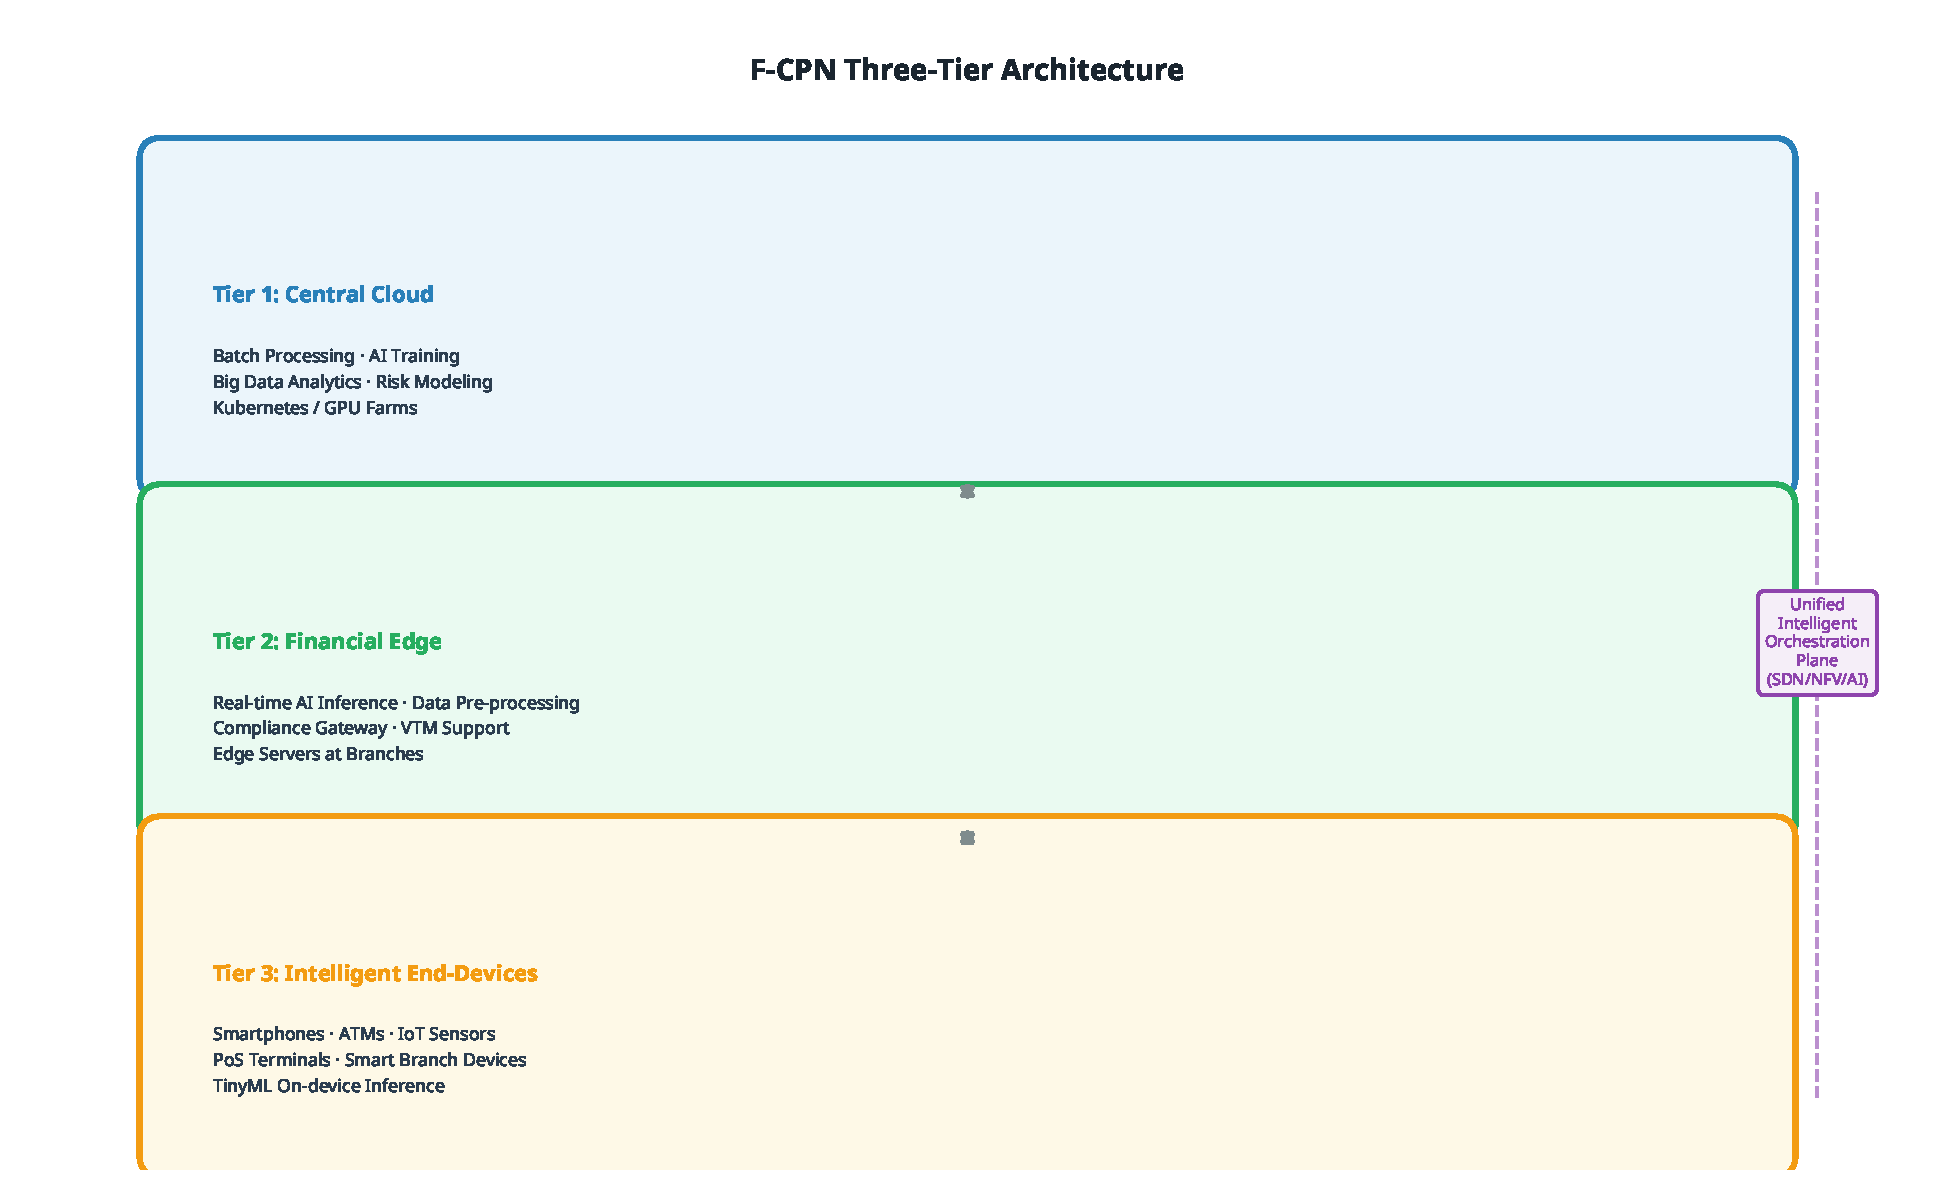
\includegraphics[width=\linewidth]{fig2_fcpn_architecture.pdf}
\end{center}
   \caption{F-CPN Conceptual Architecture}
\label{fig:architecture}
\end{figure}

\begin{itemize}
    \item \textbf{Tier 1: The Central Cloud---The Core of Strategic Intelligence and Ultimate Record.} The central cloud remains the gravitational center of the F-CPN, functioning as the "central bank" of computing power and the ultimate System of Record. Its role is to handle tasks that are compute-intensive, non-latency-sensitive, and require a global data view. This includes large-scale batch processing (e.g., end-of-day settlement), enterprise-wide data analytics, complex risk modeling, and, crucially, the training of large AI/ML models. The technology stack here comprises hyper-scale Kubernetes clusters, distributed databases, data lakes, and powerful GPU farms. While immensely powerful, its inherent distance from the end-user makes it fundamentally unsuited for real-time interaction.
    
    \item \textbf{Tier 2: The Financial Edge---The Vanguard of Real-Time Service Delivery.} The Edge is the most innovative and critical layer of the F-CPN. It consists of a distributed network of smaller-scale servers, acting as "forward-deployed warehouses" of compute. These edge nodes are strategically placed in locations with high business value and data density, such as major bank branches, regional data centers, or co-location facilities close to business districts. Their primary function is to intercept and process workloads that are latency-sensitive, data-intensive, or subject to strict data sovereignty rules. Key responsibilities include:
    \begin{itemize}
        \item \textbf{Real-time AI Inference:} Executing pre-trained models for immediate services like facial recognition, voice command processing, and real-time fraud detection.
        \item \textbf{Data Pre-processing and Aggregation:} Filtering, cleaning, and aggregating raw data streams (e.g., from video surveillance) before transmitting only the essential, structured insights to the central cloud, thus drastically reducing network load.
        \item \textbf{Compliance Gateway:} Acting as a local gateway to ensure that sensitive customer data is processed within its geographical jurisdiction, thereby satisfying regulations like PIPL.
    \end{itemize}
    Technologically, these nodes leverage lightweight container runtimes (e.g., K3s, MicroK8s), specialized AI inference accelerators, and high-speed local networking.
    
    \item \textbf{Tier 3: The Intelligent End-Device---The Point of Initial Perception and Interaction.} The final tier consists of the vast ecosystem of end-user devices, which are no longer passive terminals but active participants in the computational process. This includes everything from customer smartphones and PoS terminals to ATMs and IoT sensors within a "smart branch." These devices perform initial data capture and can run lightweight, on-device ML models for tasks like keyword spotting or basic anomaly detection. They represent the ultimate source of demand and the perception layer of the entire F-CPN.
\end{itemize}

The true power of this architecture lies in the \textbf{Unified Intelligent Orchestration Plane}. This is the network's "brain" or software-defined nervous system. It transcends the physical tiers, providing a single pane of glass for management and control. Using technologies like Software-Defined Networking (SDN) for dynamic traffic routing, Network Functions Virtualization (NFV) to deploy services as software, and an AI-driven control engine, it performs real-time, optimal scheduling. Based on telemetry data about network conditions, node utilization, and application-specific SLAs, the orchestrator decides dynamically whether a given workload should be processed on the device, at the edge, or in the cloud.

\subsection{Core Optimization Challenge: The Combinatorial Explosion of NP-Hard Problems}

The architectural blueprint of the F-CPN, while powerful, gives rise to a formidable strategic challenge: its physical layout optimization. This is not a simple technical configuration but a large-scale, discrete location-allocation problem that falls squarely into the category of NP-Hard problems. The "hardness" stems from the phenomenon of \textbf{combinatorial explosion}.

For a financial institution on the scale of ICBC, with potentially over 15,000 physical branches and office locations serving as candidate sites for edge nodes, the decision space is astronomically large. For instance, a strategic plan to deploy just 500 edge servers would require choosing 500 locations out of 15,000. The number of possible combinations is given by the binomial coefficient $\binom{15000}{500}$, a number so vast (on the order of $10^{1340}$) that it exceeds the estimated number of atoms in the observable universe. A brute-force search is not just impractical; it is a physical impossibility for any classical computer.

This inherent complexity forces us to abstract the business problem into precise mathematical formulations. We focus on two canonical yet highly relevant models that represent two sides of the same strategic coin:

\begin{itemize}
    \item \textbf{Challenge 1: Maximal Covering Location Problem (MCLP) --- The Strategic Value Maximization.} This model addresses the business question: "Given a fixed annual budget for digital infrastructure, where do we invest to achieve the maximum strategic impact?" It formalizes the problem of a phased, budget-constrained rollout. The objective is to select a predetermined number of $P$ edge locations to maximize the total volume or value of covered business demand. "Demand" here is a weighted metric that could represent transaction volume, number of high-value customers, or the density of latency-sensitive applications. Solving the MCLP provides decision-makers with a data-driven priority list for deployment, ensuring that every dollar invested yields the highest possible return in service quality and market coverage.
    
    \item \textbf{Challenge 2: Capacitated Facility Location Problem (CFLP) --- The Total Economic Efficiency.} This model tackles the holistic, long-term economic question: "What is the most cost-effective network design that guarantees service quality for all our business needs?" Unlike the MCLP, the CFLP does not fix the number of facilities. Instead, it seeks to satisfy all demands while minimizing the total cost of ownership (TCO). This TCO is a composite of the fixed Capital Expenditures (CapEx) for deploying servers and the variable Operational Expenditures (OpEx) associated with processing and data transport. The model must respect the finite processing capacity of each potential edge server. The solution to the CFLP provides the optimal, long-term blueprint for the entire network, balancing fixed costs against operational efficiency. This problem formulation is a subject of active research, with novel computational approaches constantly being explored \cite{d2023quantum}.
\end{itemize}

\begin{figure*}[htbp]
\begin{center}
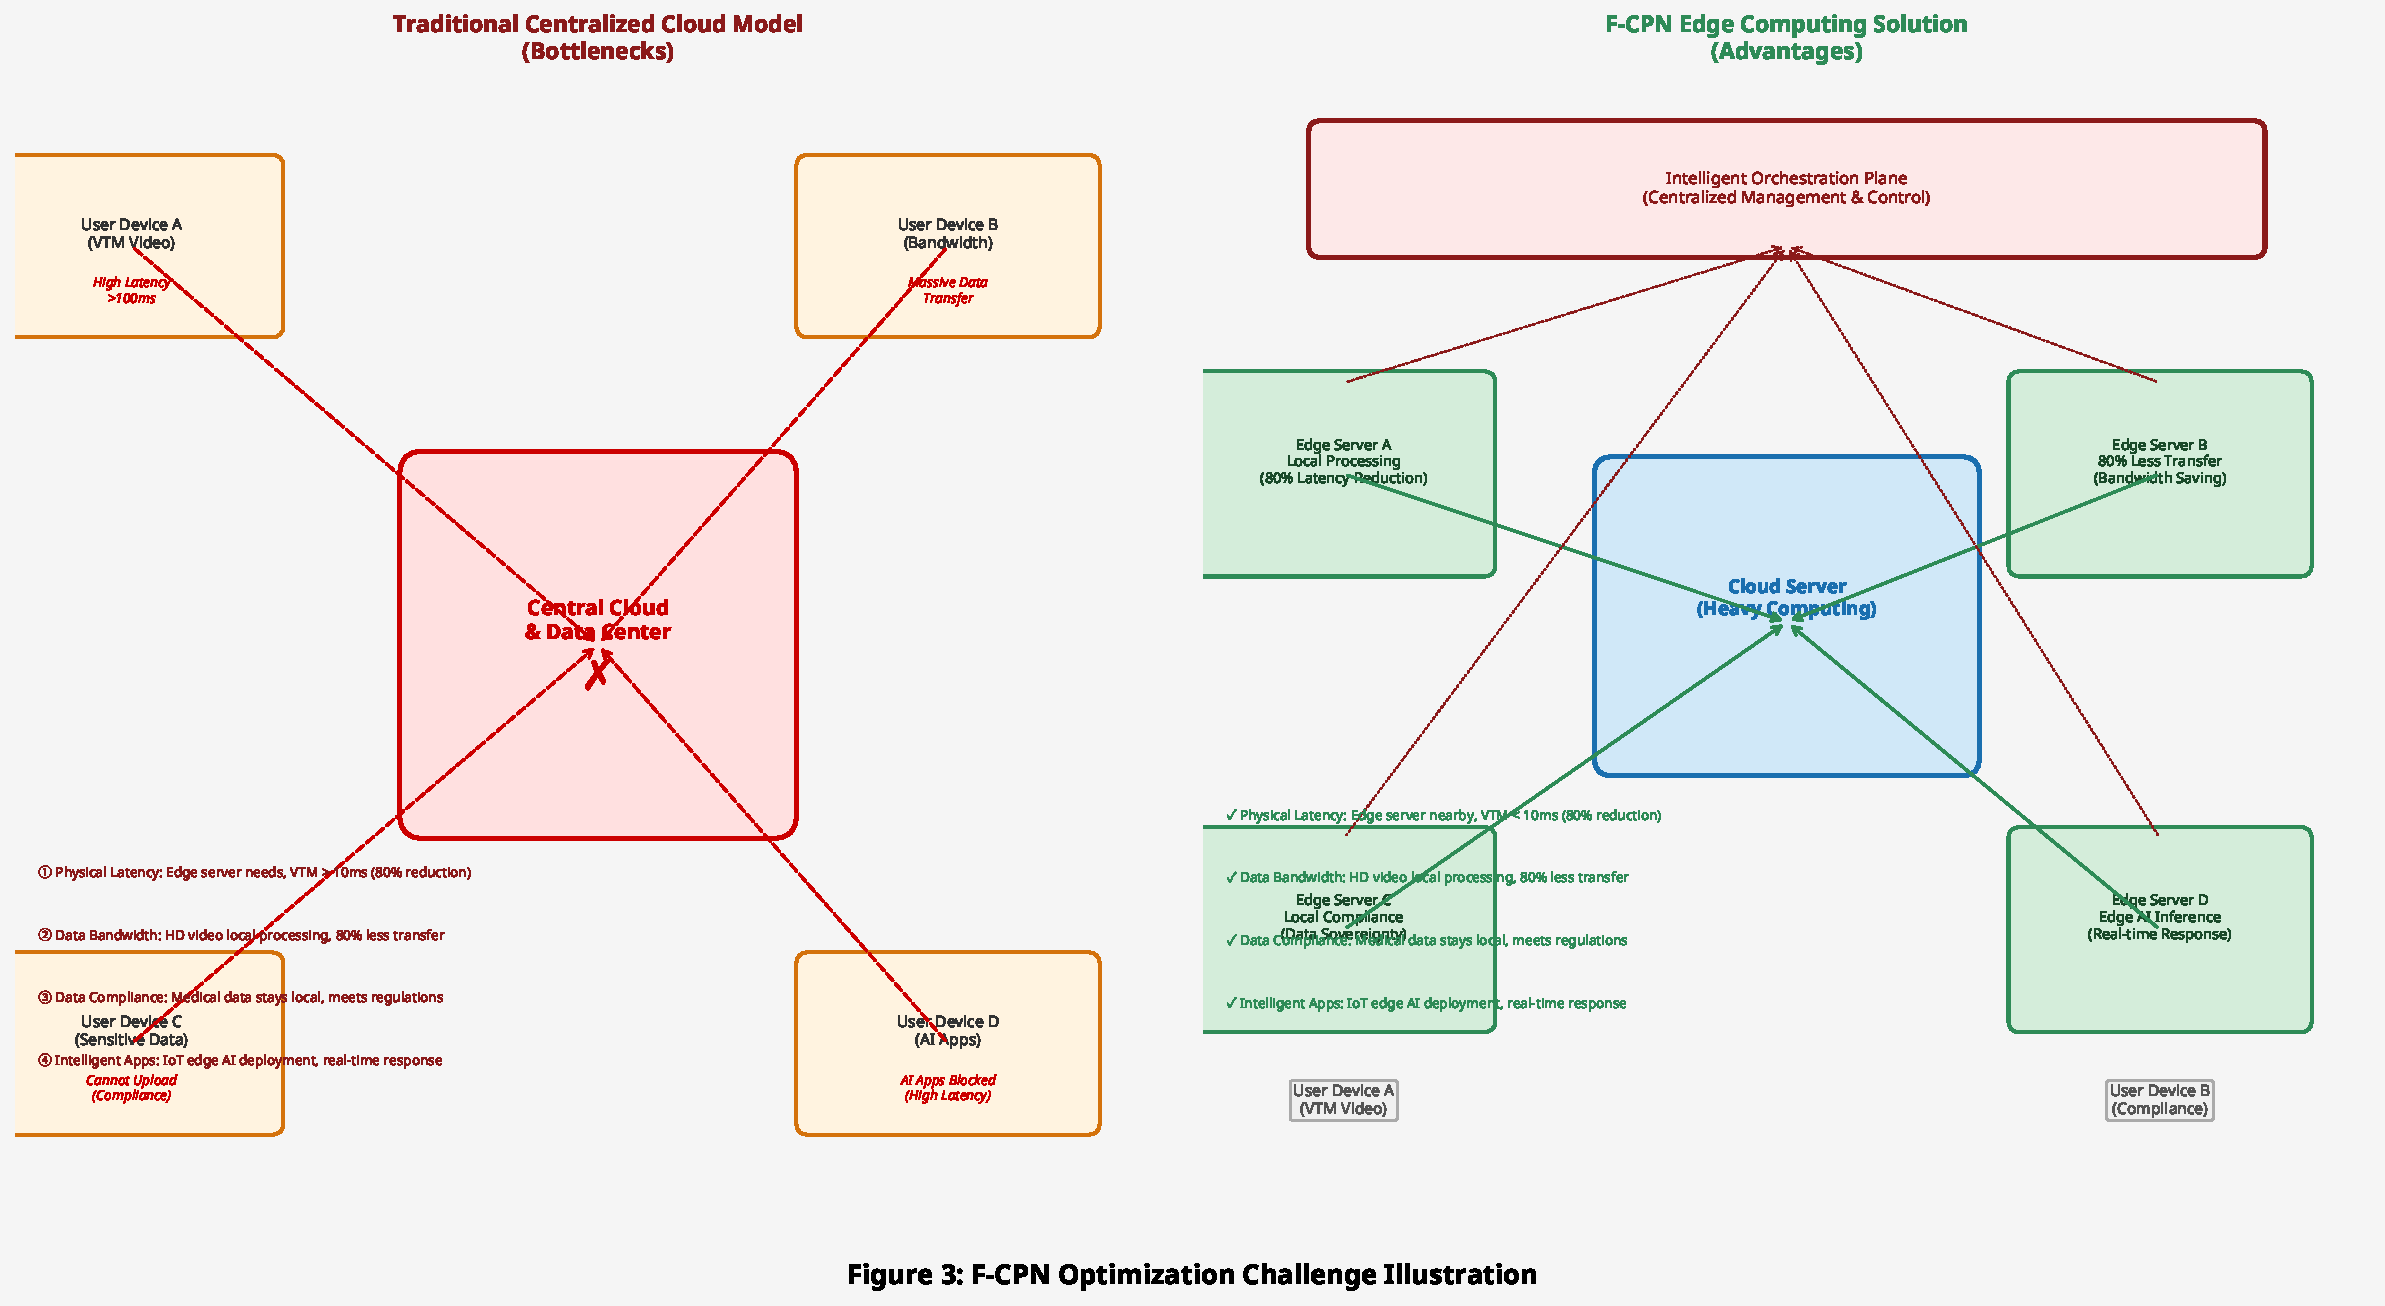
\includegraphics[width=0.9\linewidth]{fig3_optimization_challenge.pdf}
\end{center}
   \caption{F-CPN Optimization Challenge Illustration}
\label{fig:challenge}
\end{figure*}

The NP-Hard nature of these formulations means that for problems of realistic scale, finding a provably optimal solution with classical exact solvers (like Gurobi or CPLEX) can take an unacceptably long time or require prohibitive amounts of memory. This computational bottleneck is the primary motivation for exploring alternative, potentially disruptive solution paradigms, such as quantum computing.

\section{Combinatorial Optimization Modeling for F-CPN Layout}

To translate the strategic F-CN layout challenges into a solvable form, we employ the rigorous language of mathematical optimization. This section formalizes the two core problems value maximization and cost minimization into two distinct Mixed Integer Linear Programming (MILP) models. These models provide a structured framework to navigate the complex trade-offs between cost, performance, and coverage \cite{d2023quantum}.

\subsection{Model 1: Maximizing Demand Coverage (MCLP)}

This model addresses the strategic investment problem under a fixed budget, which is a common scenario in corporate capital planning. The core objective is to achieve the greatest "bang for the buck" by deploying a limited number of edge servers. We abstract the problem space into a set of discrete demand points and potential facility locations.

\subsubsection{Model Formulation}

\textbf{Sets and Parameters:}
\begin{itemize}
    \item $I$: Set of all user grid points, indexed by $i$. These points represent aggregated demand centers, such as urban residential blocks, business districts, or individual high-value corporate clients.
    \item $J$: Set of all candidate edge server locations, indexed by $j$. These are potential sites for deployment, typically corresponding to ICBC's existing physical assets like branches or regional offices.
    \item $d_i$: Computing demand at user point $i$. This crucial parameter is a weighted metric reflecting not just raw transaction volume, but also the strategic value and latency-sensitivity of the services required at that point.
    \item $R$: Effective coverage radius of an edge server. This parameter defines the geographical or network-latency boundary within which an edge server can provide the required low-latency service (e.g., under 10ms RTT).
    \item $N_i = \{j \in J \mid \text{distance}(i, j) \le R\}$: Pre-computed set of candidate servers that can cover user point $i$. This simplifies the model by encoding the geographical constraints directly.
    \item $P$: Total number of edge servers to be deployed, representing the fixed budget constraint.
\end{itemize}

\textbf{Decision Variables:}
\begin{itemize}
    \item $x_j \in \{0, 1\}$: The primary location variable. A value of 1 signifies a strategic decision to open an edge server at location $j$; 0 otherwise.
    \item $z_i \in \{0, 1\}$: The coverage status variable. A value of 1 indicates that the demand at point $i$ is successfully covered by at least one deployed edge server; 0 otherwise.
\end{itemize}

\textbf{Objective Function:} The goal is to maximize the total weighted demand of all covered user points.
\begin{equation}
\max \sum_{i \in I} d_i z_i
\end{equation}

\textbf{Constraints:} The model is subject to the following logical and physical limitations:
\begin{align}
\sum_{j \in J} x_j &= P \label{eq:mclp_p} \\
z_i &\le \sum_{j \in N_i} x_j, \quad &\forall i \in I \label{eq:mclp_cov} \\
x_j &\in \{0, 1\}, \quad &\forall j \in J \label{eq:mclp_xj} \\
z_i &\in \{0, 1\}, \quad &\forall i \in I \label{eq:mclp_zi}
\end{align}

\subsubsection{Analysis of the MCLP Model}

The elegance of this formulation lies in its directness. The objective function (1) clearly aligns with the business goal of maximizing market impact. Constraint (\ref{eq:mclp_p}) is the hard budget constraint, enforcing that exactly $P$ facilities are opened. The key logical link is Constraint (\ref{eq:mclp_cov}), which states that a demand point $i$ can only be considered covered ($z_i = 1$) if at least one server is opened within its coverage neighborhood $N_i$. This "big M"-style constraint elegantly connects the location decisions ($x_j$) to the coverage outcomes ($z_i$). The binary nature of the variables, defined in (\ref{eq:mclp_xj}) and (\ref{eq:mclp_zi}), makes this a classic NP-Hard integer programming problem.

\subsection{Model 2: Minimizing Total Deployment and Operational Cost (CFLP)}

This model addresses the more comprehensive, long-term economic question of designing the most cost-efficient network that satisfies all service demands. It moves beyond simple coverage to include detailed operational costs and capacity limits, providing a holistic view of the Total Cost of Ownership (TCO). This formulation explicitly models the hybrid nature of the F-CPN, allowing demand to be served by either a local edge server or the central cloud.

\subsubsection{Model Formulation}

\textbf{Additional Parameters:}
\begin{itemize}
    \item $C_{\text{fix},j}$: Fixed cost (CapEx) to open and equip an edge server at location $j$.
    \item $C_{\text{var},j}^{\text{edge}}$: Variable cost (OpEx) per unit of demand processed at edge server $j$. This includes power, cooling, and local maintenance.
    \item $C_{\text{var}}^{\text{cloud}}$: Variable cost per unit of demand processed at the central cloud.
    \item $C_{\text{tran},ij}$: Cost to transport a unit of demand from user $i$ to edge server $j$. This is a function of network distance and bandwidth price.
    \item $C_{\text{tran},i}^{\text{cloud}}$: Cost to transport a unit of demand from user $i$ directly to the cloud.
    \item $C_{\text{tran},j}^{\text{cloud}}$: Cost to transport a unit of offloaded demand from edge $j$ to the cloud (backhaul cost).
    \item $K_j$: Maximum processing capacity of the edge server at location $j$. This reflects the physical hardware limitations.
\end{itemize}

\textbf{Additional Decision Variables:}
\begin{itemize}
    \item $y_{ij} \in \{0, 1\}$: An assignment variable, where 1 means user $i$'s demand is assigned to edge server $j$.
    \item $y_i^{\text{cloud}} \in \{0, 1\}$: An assignment variable, where 1 means user $i$'s demand is assigned to the cloud.
    \item $u_j \ge 0$: A continuous variable representing the amount of demand offloaded from an overloaded edge server $j$ to the cloud.
\end{itemize}

\textbf{Objective Function:} The objective is to minimize the total system-wide cost, which is the sum of fixed deployment costs and all variable processing and transport costs.
\begin{align}
\min \quad &\sum_{j \in J} C_{\text{fix},j} x_j \nonumber \\
&+ \sum_{i \in I} \sum_{j \in J} \left(C_{\text{var},j}^{\text{edge}} + C_{\text{tran},ij}\right) d_i y_{ij} \nonumber \\
&+ \sum_{i \in I} \left(C_{\text{var}}^{\text{cloud}} + C_{\text{tran},i}^{\text{cloud}}\right) d_i y_i^{\text{cloud}} \nonumber \\
&+ \sum_{j \in J} \left(C_{\text{var}}^{\text{cloud}} + C_{\text{tran},j}^{\text{cloud}}\right) u_j \label{eq:cflp_obj}
\end{align}

\textbf{Constraints:} The cost minimization is subject to ensuring all demands are met and capacities are respected.
\begin{align}
\sum_{j \in J} y_{ij} + y_i^{\text{cloud}} &= 1, \quad &\forall i \in I \label{eq:cflp_assign} \\
y_{ij} &\le x_j, \quad &\forall i \in I, j \in J \label{eq:cflp_link} \\
\sum_{i \in I} d_i y_{ij} &\le K_j + u_j, \quad &\forall j \in J \label{eq:cflp_cap} \\
x_j, y_{ij}, y_i^{\text{cloud}} &\in \{0, 1\}, \quad &\forall i \in I, j \in J \label{eq:cflp_bin} \\
u_j &\ge 0, \quad &\forall j \in J \label{eq:cflp_cont}
\end{align}

\subsubsection{Analysis of the CFLP Model}

This model presents a much more detailed and nuanced view. The objective function (\ref{eq:cflp_obj}) is a comprehensive TCO calculation, breaking down costs into four components: fixed deployment, edge processing and transport, direct-to-cloud processing, and edge-to-cloud offloading. This structure allows for fine-grained economic analysis.

The constraints enforce the operational logic. Constraint (\ref{eq:cflp_assign}) is a critical service guarantee, ensuring that every single demand point is assigned to exactly one service provider (either an edge server or the cloud). Constraint (\ref{eq:cflp_link}) is the fundamental link between opening a facility and assigning demand to it; no demand can be sent to a non-existent server. Finally, Constraint (\ref{eq:cflp_cap}) is the capacity logic. It uniquely allows for "soft" capacity by introducing the offloading variable $u_j$, which provides the model with the flexibility to handle demand spikes by offloading excess load to the cloud, albeit at a higher cost captured in the objective function. This makes the model more robust and reflective of a real-world, elastic infrastructure. The mix of binary and continuous variables makes this a challenging MILP, whose solution represents the economically optimal state of the entire F-CPN.

\section{Quantum Computing: A Disruptive Paradigm for F-CPN Optimization}

The NP-Hard nature of the MCLP and CFLP models presents a significant computational bottleneck. For a network on the scale of ICBC, classical exact algorithms (like Branch and Bound used in solvers such as Gurobi or CPLEX) scale exponentially in time and memory, often failing to find an optimal solution within a reasonable timeframe. While heuristic and metaheuristic algorithms (like Genetic Algorithms or Simulated Annealing) can find good approximate solutions more quickly, they do not guarantee optimality and can easily get trapped in local optima.

To break through this computational ceiling, we turn to the frontier of quantum computing. Specifically, we explore Quantum Annealing (QA), a specialized form of quantum computing designed explicitly to solve complex combinatorial optimization problems by exploiting the principles of quantum mechanics.

\subsection{The Principles of Quantum Annealing}

Quantum Annealing operates on a fundamentally different physical principle than classical computing. Instead of manipulating bits (0s and 1s) through logical gates, QA uses quantum bits (qubits) that can exist in a superposition of states (both 0 and 1 simultaneously). The process relies on two key quantum phenomena:

\begin{enumerate}
    \item \textbf{Quantum Superposition:} This allows the quantum processor to explore a vast number of potential solutions simultaneously, rather than sequentially as a classical computer must do.
    \item \textbf{Quantum Tunneling:} In a complex optimization landscape characterized by many local minima (valleys), a classical algorithm (like simulated annealing) must "climb" over the energy barriers (hills) to escape a local minimum. This requires thermal energy and time. Quantum tunneling, however, allows the system to literally "tunnel" through these high-energy barriers directly to a lower-energy state (a better solution), drastically accelerating the search for the global minimum.
\end{enumerate}

The physical process of quantum annealing involves defining an energy landscape (a Hamiltonian) that corresponds to the optimization problem. The system is initialized in the known ground state (lowest energy state) of a simple Hamiltonian. Then, the system is slowly and continuously evolved until the Hamiltonian represents the complex problem we want to solve. According to the Adiabatic Theorem of quantum mechanics, if this evolution is slow enough, the system will remain in the ground state throughout the process. The final state of the qubits then represents the optimal solution to the problem.

\subsection{Mapping the F-CPN Models to QUBO}

To solve our MCLP and CFLP models on a quantum annealer (like those built by D-Wave Systems), we must first translate them into a specific mathematical format: Quadratic Unconstrained Binary Optimization (QUBO).

A QUBO problem seeks to minimize a quadratic objective function of binary variables, without any explicit constraints. The general form is:
\begin{equation}
\min_{x \in \{0,1\}^n} \sum_{i} Q_{ii} x_i + \sum_{i < j} Q_{ij} x_i x_j
\end{equation}
where $x$ is a vector of binary variables and $Q$ is an upper-triangular matrix of real weights.

The transformation from our constrained MILP models to an unconstrained QUBO model involves two main steps, illustrated in Figure \ref{fig:qubo}:

\begin{figure}[htbp]
\begin{center}
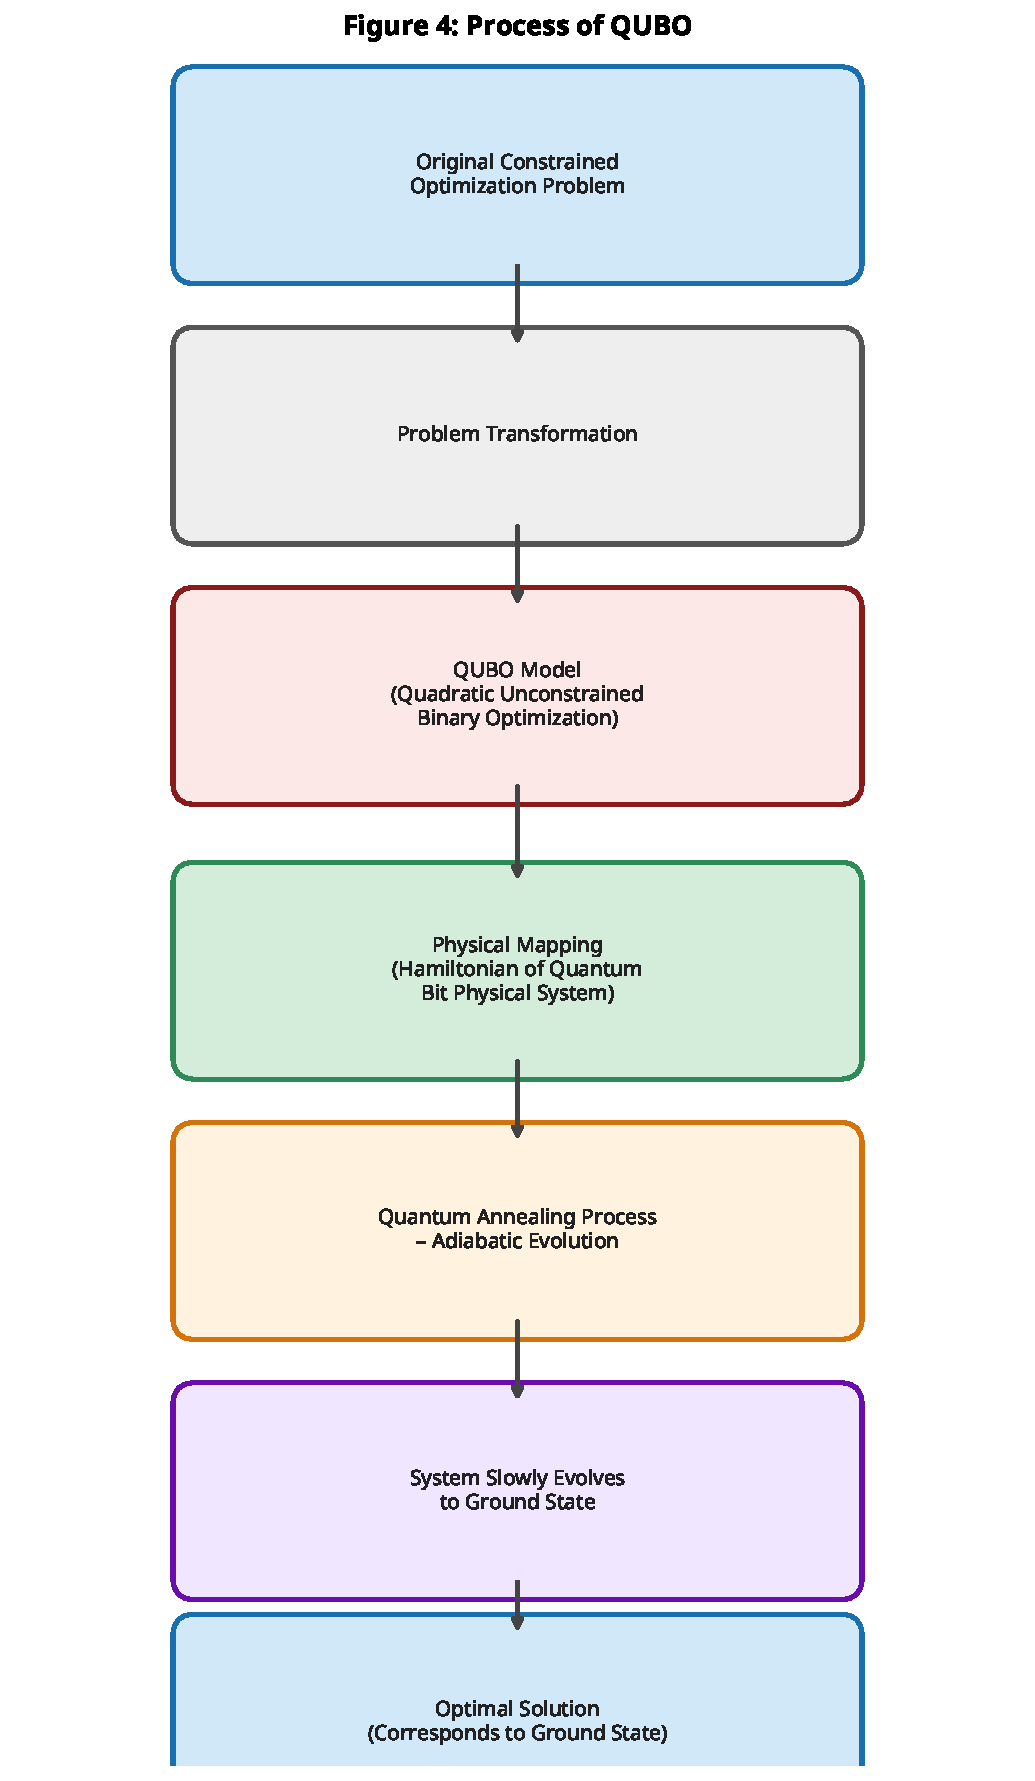
\includegraphics[width=0.8\linewidth]{fig4_qubo_process.pdf}
\end{center}
   \caption{Process of QUBO}
\label{fig:qubo}
\end{figure}

\textbf{Step 1: Handling Constraints via Penalty Methods.} The most significant challenge is that QUBO, by definition, cannot have constraints like equations (\ref{eq:mclp_p}) or (\ref{eq:cflp_assign}). We must convert these hard constraints into "soft" penalties added to the objective function. For example, the budget constraint $\sum_{j \in J} x_j = P$ in the MCLP model is transformed into a penalty term:
\begin{equation}
\lambda \left( \sum_{j \in J} x_j - P \right)^2
\end{equation}
where $\lambda$ is a large positive penalty coefficient. If the constraint is violated, this term adds a massive penalty to the objective function, making that solution highly unfavorable. If the constraint is satisfied, the term evaluates to zero.

\textbf{Step 2: Discretizing Continuous Variables.} The CFLP model contains continuous variables ($u_j$) for capacity offloading. QUBO only accepts binary variables. Therefore, we must discretize $u_j$ using a binary expansion. We represent $u_j$ as a sum of binary variables multiplied by powers of 2 (or other chosen bases):
\begin{equation}
u_j \approx \sum_{k=0}^{K} 2^k w_{jk}
\end{equation}
where $w_{jk} \in \{0, 1\}$. This approximation increases the number of variables (qubits) required but allows the continuous aspect of the problem to be mapped onto the quantum hardware.

By applying these transformations, the complex, constrained F-CPN layout models are rewritten as a single, large QUBO matrix $Q$. This matrix is then directly programmed into the quantum annealer, where the physical interactions between the qubits are set according to the weights in $Q$.

\subsection{Physical Solution: The Quantum Annealing Process}

Once the QUBO formulation is complete, it is mapped onto the physical qubits of the quantum annealer. This mapping translates the mathematical problem into a physical system whose energy landscape corresponds to the objective function. The core of the annealing process is governed by a time-dependent Hamiltonian, $\mathcal{H}(t)$, which describes the total energy of the quantum system at any given time $t$:

\begin{equation}
\mathcal{H}(t) = A(t) \mathcal{H}_{\text{initial}} + B(t) \mathcal{H}_{\text{problem}}
\end{equation}

Here, $\mathcal{H}_{\text{initial}}$ is a simple Hamiltonian whose ground state is easy to prepare (typically representing a state where all qubits are in a superposition of 0 and 1). $\mathcal{H}_{\text{problem}}$ is the Hamiltonian that encodes our QUBO matrix $Q$. The functions $A(t)$ and $B(t)$ are the annealing schedules. At the start of the process ($t=0$), $A(0)$ is large and $B(0)$ is near zero, so the system is dominated by the initial, simple state. As time progresses to the total annealing time $T_a$, $A(t)$ gradually decreases to zero, while $B(t)$ increases to a maximum value. By the end of the process ($t=T_a$), the system is entirely governed by $\mathcal{H}_{\text{problem}}$.

According to the adiabatic theorem, if this transition is performed sufficiently slowly, the system will remain in its ground state throughout the evolution. Therefore, the final state of the qubits represents the global minimum of $\mathcal{H}_{\text{problem}}$, which corresponds to the optimal solution of our F-CPN layout problem. Figure \ref{fig:annealing} illustrates the complete algorithmic flow from the original problem to the quantum measurement.

\begin{figure}[htbp]
\begin{center}
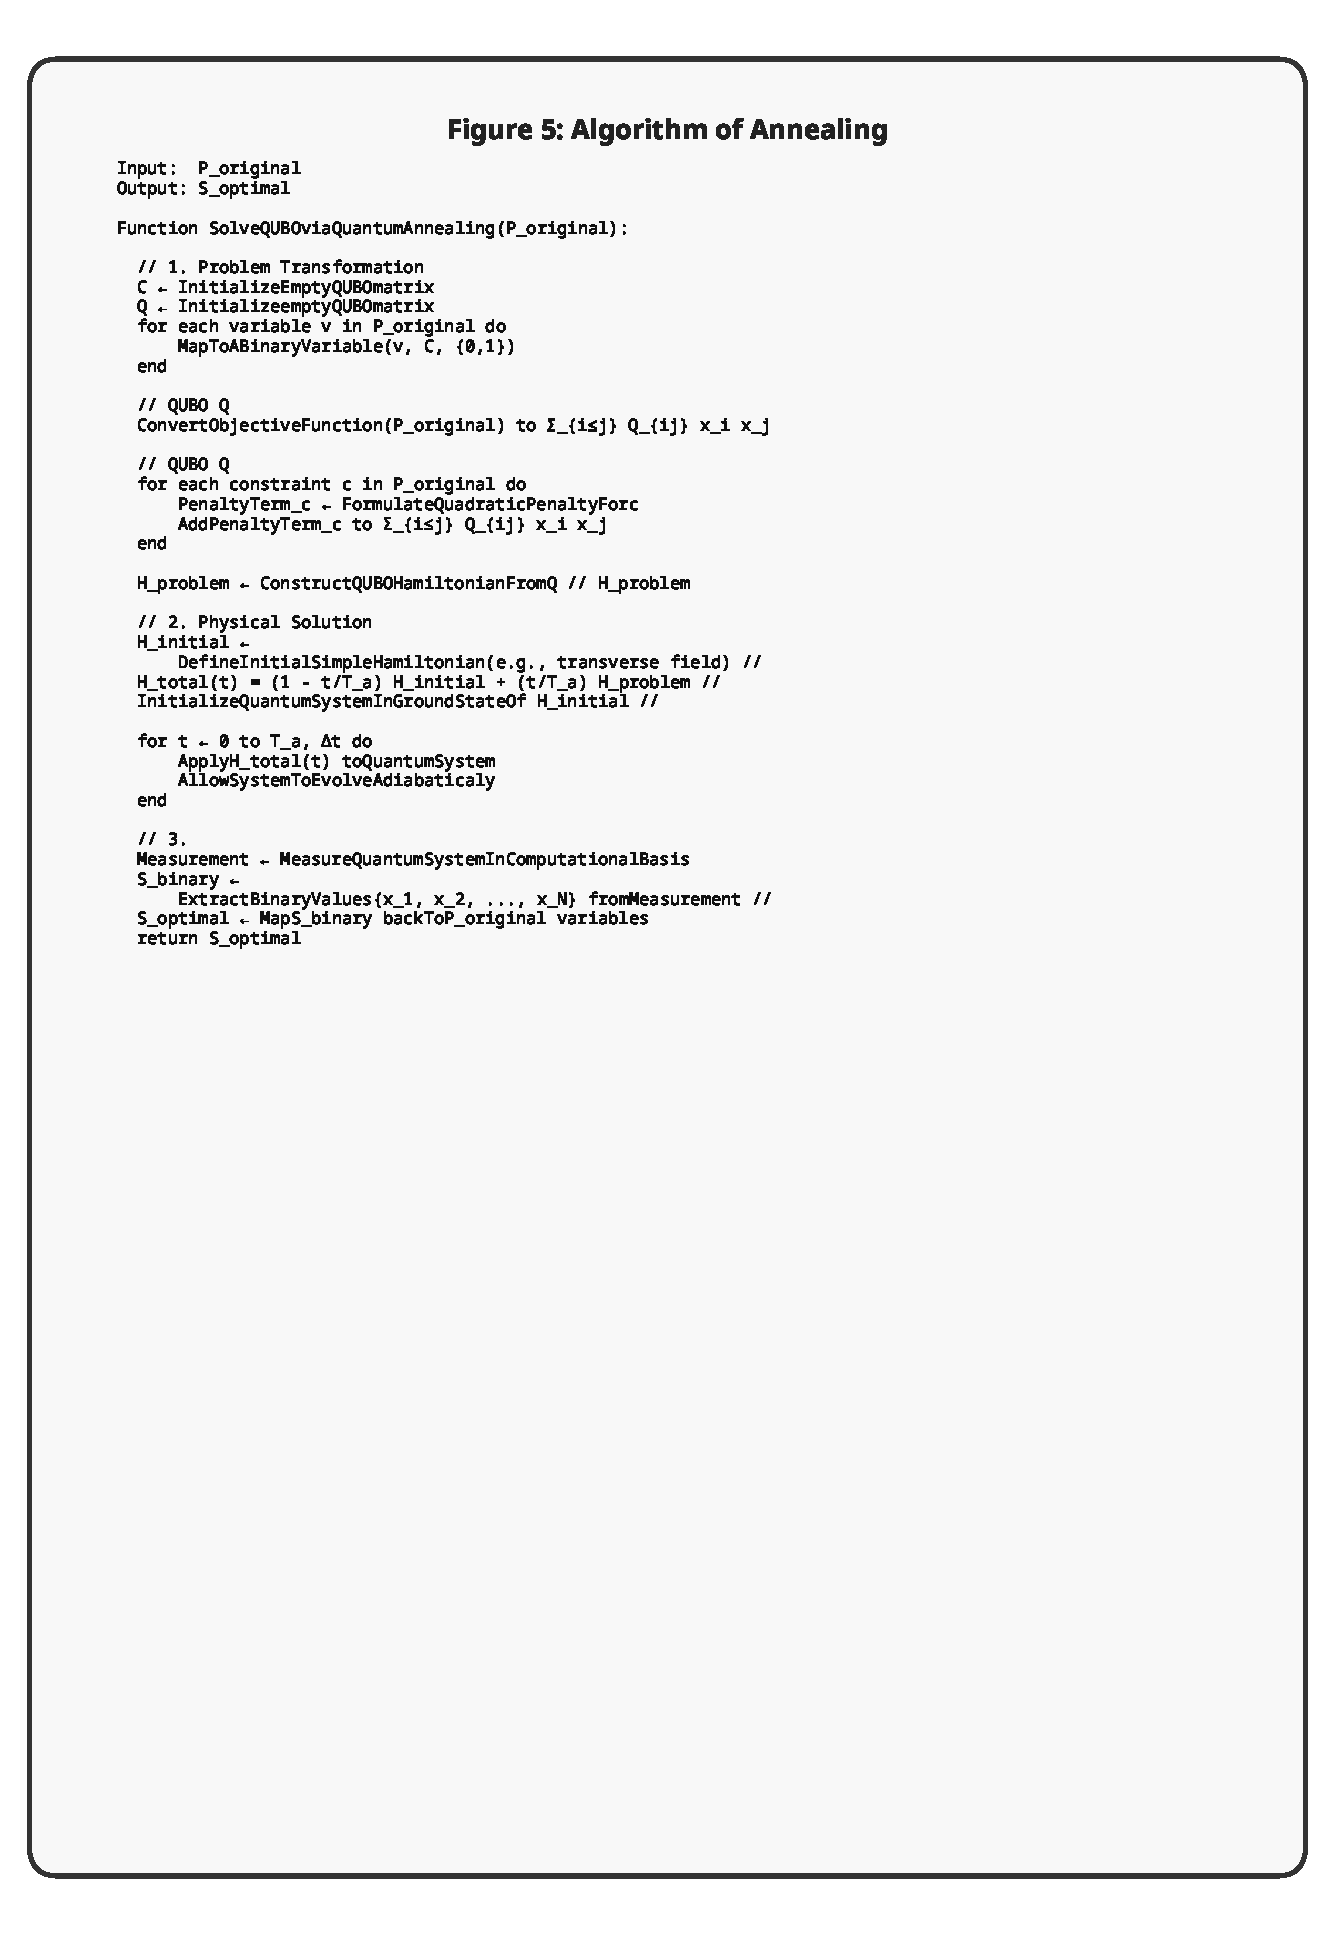
\includegraphics[width=0.8\linewidth]{fig5_annealing_algorithm.pdf}
\end{center}
   \caption{Algorithm of Annealing}
\label{fig:annealing}
\end{figure}

\section{Quantum Computing in Finance: From Optimization to Simulation}

The application of quantum computing in the financial sector extends far beyond the layout optimization of IT infrastructure. As financial markets become increasingly complex and data-driven, the computational demands of risk management, derivative pricing, and portfolio optimization are pushing classical computers to their limits. Quantum computing offers a fundamentally new paradigm, categorized primarily into two pillars: Quantum Optimization and Quantum Simulation.

\subsection{Studies in Quantum Optimization for Finance}

Quantum optimization, particularly using Quantum Annealing or the Quantum Approximate Optimization Algorithm (QAOA) on gate-model computers, is highly applicable to problems that can be framed as finding the best combination from a vast set of possibilities.

\textbf{Case Study 1: Portfolio Optimization.} The classic Markowitz portfolio theory seeks to maximize expected return for a given level of risk (variance). This is a quadratic optimization problem. In a quantum context, the objective function can be mapped directly to a QUBO formulation:
\begin{equation}
\min_x \left( - \sum_{i} \mu_i x_i + \gamma \sum_{i,j} \sigma_{ij} x_i x_j \right)
\end{equation}
where $x_i$ are binary variables representing the inclusion of asset $i$, $\mu_i$ is the expected return, $\sigma_{ij}$ is the covariance matrix, and $\gamma$ is a risk aversion parameter. Quantum annealers can explore the vast combinatorial space of asset selections much more efficiently than classical solvers, especially when dealing with hundreds or thousands of assets and complex constraints like transaction costs or minimum holding periods.

\textbf{Case Study 2: Transaction Settlement and Cash Management.} Large financial institutions process millions of transactions daily, requiring complex settlement and clearing processes. These processes often involve finding optimal cycles or netting arrangements within a network of counter-parties to minimize liquidity requirements. This can be modeled as a graph optimization problem (e.g., finding the optimal set of edges to clear). Quantum algorithms have shown promise in identifying these optimal netting cycles faster, thereby freeing up trapped capital and reducing systemic risk.

\subsection{The Frontier: Risk Analysis and Derivative Pricing}

Beyond optimization, quantum simulation---leveraging the principles of quantum mechanics to simulate complex stochastic processes---holds immense potential for risk analysis and pricing.

\textbf{Case Study 3: Credit Risk Analysis and Value at Risk (VaR).} Calculating VaR for a large, complex portfolio typically requires massive Monte Carlo simulations to model the distribution of potential future losses under various market scenarios. Classical Monte Carlo simulations converge at a rate of $O(1/\sqrt{N})$, where $N$ is the number of samples. Quantum Amplitude Estimation (QAE) algorithms can theoretically achieve a quadratic speedup, converging at $O(1/N)$. This means a quantum computer could calculate VaR significantly faster or with much higher precision in the same amount of time, allowing banks to respond to market volatility in near real-time.

\textbf{Case Study 4: Derivative Pricing.} The pricing of complex, path-dependent derivatives (like Asian options or barrier options) also relies heavily on Monte Carlo methods to simulate the underlying asset's price trajectory. Similar to VaR calculations, QAE can accelerate these simulations. Furthermore, quantum computers can potentially model the underlying stochastic differential equations (SDEs) more naturally, capturing complex market dynamics (like stochastic volatility or jump-diffusion models) that are difficult to simulate classically.

\subsection{A Realistic Outlook: The NISQ Era and Beyond}

While the theoretical potential is vast, it is crucial to acknowledge the current state of the technology. We are currently in the Noisy Intermediate-Scale Quantum (NISQ) era. Today's quantum processors have a limited number of qubits, and these qubits are prone to errors (decoherence) caused by environmental noise.

Therefore, the immediate future of quantum finance will likely be characterized by \textbf{hybrid quantum-classical algorithms}. In these approaches, a classical computer handles the bulk of the data processing and problem setup, while the quantum processor acts as a specialized co-processor (a Quantum Processing Unit, or QPU) to tackle the most computationally intractable kernel of the problem. For example, in our F-CPN layout problem, a classical algorithm might partition the network into smaller regions, and the quantum annealer would solve the layout problem for each region.

\section{Conclusion and Strategic Outlook}
\label{sec:conclusion}

This paper has systematically addressed the pressing need for ICBC to evolve its IT infrastructure beyond the limitations of the centralized cloud. We have introduced the Financial Computing Power Network (F-CPN) as a necessary, three-tiered architectural paradigm designed to meet the demands of latency, bandwidth, and compliance in the Digital 2.0 era. By formalizing the strategic layout of this network into rigorous mathematical models (MCLP and CFLP), we have provided a structured methodology for balancing investment, coverage, and total cost of ownership.

Recognizing the NP-Hard complexity of these optimization problems, we have explored the disruptive potential of quantum computing, specifically quantum annealing via the QUBO framework, as a viable solution path. Furthermore, we have contextualized this within the broader landscape of quantum finance, highlighting applications in portfolio optimization, risk analysis, and derivative pricing.

To translate these findings into actionable strategy, we propose two core recommendations for ICBC:

\begin{enumerate}
    \item \textbf{Launch a Focused F-CPN Optimization Pilot Project:} ICBC should initiate a pilot program to apply the MCLP and CFLP models to a specific, high-value regional network (e.g., a major metropolitan area). This pilot should utilize classical solvers to establish a baseline, while concurrently partnering with quantum hardware providers (or utilizing quantum cloud services) to test the QUBO formulations on actual quantum annealers. This will provide empirical data on the performance and cost-effectiveness of the F-CPN architecture and the viability of quantum solutions in a real-world banking context.
    \item \textbf{Cultivate Quantum-Ready Capabilities as a Long-Term Strategic Hedge:} While fault-tolerant, large-scale quantum computers are still years away, the financial industry is rapidly moving towards "quantum readiness." ICBC must actively build internal expertise in quantum algorithms and hybrid quantum-classical architectures. This involves training specialized personnel, developing quantum-inspired classical algorithms, and identifying the specific business processes (like complex derivative pricing or large-scale risk modeling) that will benefit most from future quantum acceleration. By doing so, ICBC will position itself not just to react to the quantum revolution, but to lead it.
\end{enumerate}

{\small
\bibliographystyle{ieee}
\begin{thebibliography}{10}\itemsep=-1pt

\bibitem{firat2023future}
U.~Firat, \emph{The Future of Banking: A Comprehensive Analysis of Digital Transformation and FinTech Integration}. Journal of Financial Technology, 2023.

\bibitem{ross2019designed}
J.~W. Ross, C.~M. Beath, and M.~Mocker, \emph{Designed for Digital: How to Architect Your Business for Sustained Success}. MIT Press, 2019.

\bibitem{ometov2022survey}
A.~Ometov et~al., \emph{A Survey on Multi-Access Edge Computing for the Internet of Things}. IEEE Communications Surveys \& Tutorials, 2022.

\bibitem{liu2023computing}
Y.~Liu et~al., \emph{Computing Power Network: A Survey}. IEEE Access, 2023.

\bibitem{d2023quantum}
M.~D'Amato et~al., \emph{Quantum Computing for Combinatorial Optimization in Finance}. Quantitative Finance, 2023.

\bibitem{markowitz1952portfolio}
H.~Markowitz, \emph{Portfolio Selection}. The Journal of Finance, 1952.

\bibitem{bouland2020prospects}
A.~Bouland et~al., \emph{Prospects and Challenges of Quantum Finance}. Nature Reviews Physics, 2020.

\end{thebibliography}
}

\end{document}
